% included from comp for modification for possible inclusion
%.... included from comp for modification for possible inclusion
A particle that is incident in a PbWO$_{4}$ crystal will produce an electromagnetic shower of lower energy electron/positron pairs and photons. The showering particles will ultimately dissipate their energy through ionization, leading to the excitation of the scintillating centers of the PbWO$_{4}$ crystal. The scintillating centers will de-excite producing a pulse of scintillating light at a specific wavelength that is proportional to the energy of the original, incident particle. This pulse of light is enhanced and converted to an analog signal by the APD and VPT sensors.
%This pulse of light is enhanced and converted to an analog signal by the avalanche photodiodes, in the barrel, and vacuum phototriodes, in the end-caps, sensors.

The front-end electronics of the EB and EE use 12-bit analog-to-digital converters to sample the analog signals at 25 ns intervals. Ten consecutive amplitude samples are stored for each recorded pulse in a crystal. In the front-end electronics of the ECAL, the signal from the photo-detectors is amplified and shaped, thereby defining the shape of the pulse \cite{Karimäki:368412}. This shape is constant for all sampled pulses and is very well known. In Figure~\ref{tec_pulseshape} the time structure of a typical signal pulse shape as measured after amplification (solid line) is shown. The normalized amplitude of the pulse, $A/A_{max}$, is a function of the time difference T-T$_{max}$, where T$_{max}$ is defined as the time when the pulse reaches its maximum value. The dots are the ten discrete samples of the pulse, as typical in a single event, with the pedestal amplitude subtracted and normalized to the maximum amplitude. 

For a given electronic channel, this exact pulse shape is obtained, to a very good approximation, for all types of particles and for all momenta. The amplitude of the pulse, for any given sample, is proportional to the energy deposited by the originating particle in a crystal. The delays in the EB/EE readout pipelines, common for the 5x5 crystal towers used to group crystals in the ECAL, are adjusted in steps of 1.04 ns such that the signal pulse is expected to start from the fourth sample and the baseline pedestal amplitude can be estimated from the first three samples \cite{CMS-NOTE-2010-012}. The rising part of the shaped pulse depends on the relaxation time of the PbWO$_{4}$ crystal scintillation process, while the falling part of the pulse is determined by the time constants of the front-end electronics.

\begin{figure}[htbp]
\begin{center}
\resizebox{0.75\linewidth}{!}{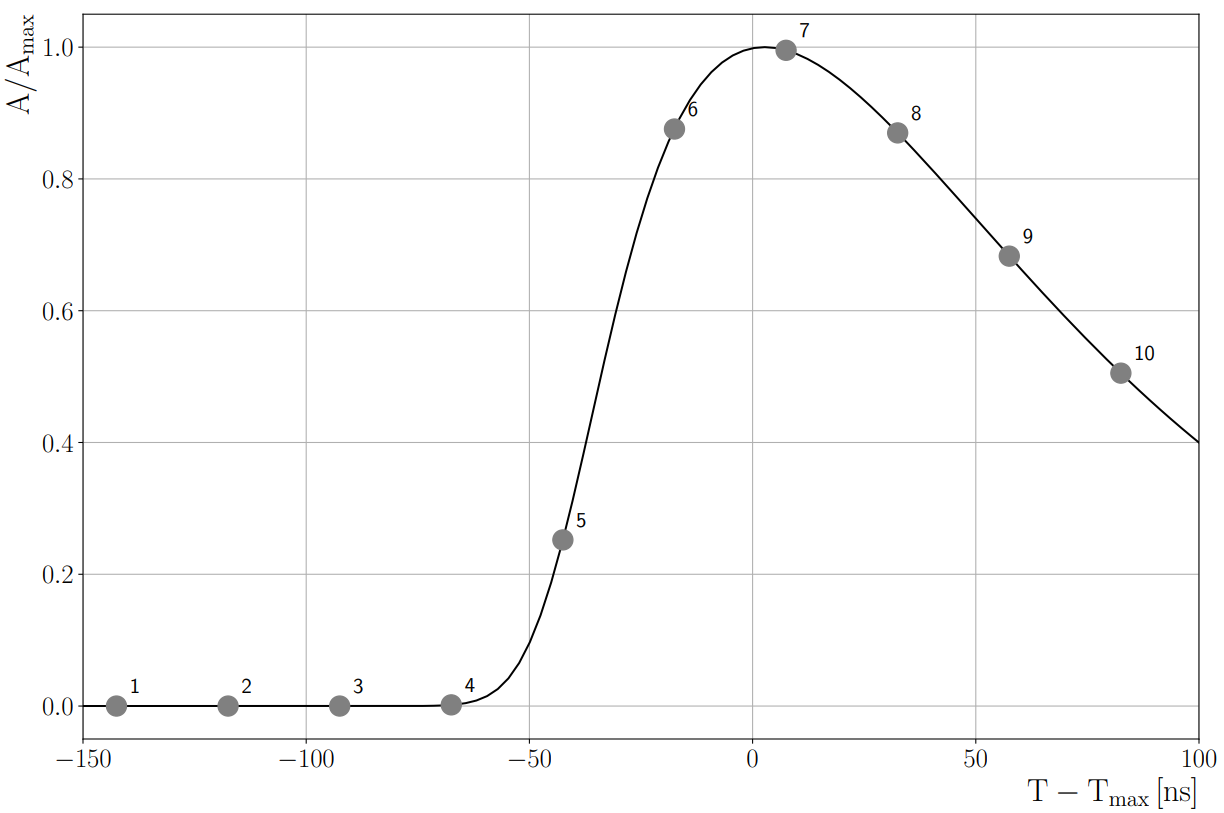
\includegraphics{fig/sec_reco/pulse_template.png}}
\caption{The typical pulse shape measured in the ECAL, as a function of the difference between the time (T) of the ADC sample and the time (Tmax) of the maximum of the pulse and the amplitude of the pulse (A) normalized by the maximum amplitude of the pulse (A$_{max}$).  The dots indicate ten discrete samples of the pulse as taken from a single event with the pedestal subtracted.}
\label{tec_pulseshape}
\end{center}
\end{figure}

\begin{equation}\label{en-wt}
A = \sum^{N}_{i=1} w_{i} x S_{i}\qquad
\end{equation}
%In equation ~\ref{en-wt} $A$ is the pulse amplitude, $N$ is the number of samples, and $S_{i}$ is the pulse height of the sample. The weights $w_{i}$ are determined, per crystal, periodically through an offline calibration \cite{Adzic:1009081}.

The maximum amplitude of the measured pulse has been reconstructed using two different methods over the operation of the CMS experiment. During LHC Run I, from 2009 through 2013, a weights algorithm was used, and with this method the pulse amplitude is estimated as the linear combination of the ten sampled amplitudes multiplied by a predetermined weight specific to a particular sample as shown in Equation~\ref{en-wt}. Here $A$ is the total pulse amplitude, $N$ is the number of samples, $S_{i}$ are the sampled pulse amplitudes, and $w_{i}$ are the weights. The values for $w_{i}$ where determined, by channel, periodically through an offline calibration \cite{Adzic:1009081}.

\hfill
\begin{figure}[htbp]
\begin{center}
\resizebox{0.75\linewidth}{!}{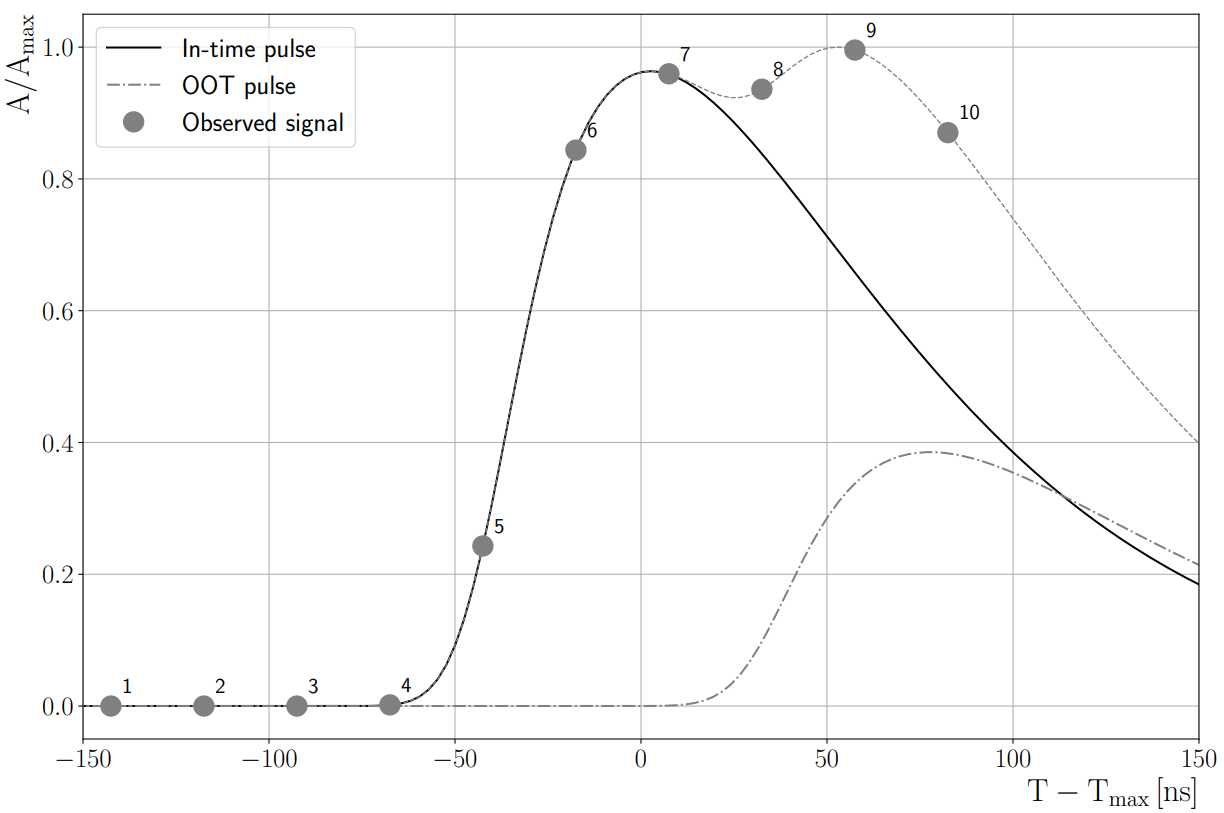
\includegraphics{fig/sec_reco/two_pulses.png}}
\caption{The fitted pulse for a simulated event with twenty average pileup events and 25 ns bunch spacing as a function of the difference between the time (T) of the ADC sample and the time (Tmax) of the maximum of the pulse and the amplitude of the pulse (A) normalized by the maximum amplitude of the pulse (A$_{max}$). The dots represent the 10 discrete samples of the measured pulse shape (dashed line) that is a superposition of an in-time pulse (solid line) and an OOT pulse (dashed line). 
%Note that the samples are numbered starting at 0 instead of 1. 
}
\label{tec_multifit2}
\end{center}
\end{figure}

During LHC Run II, from 2015 through 2018, the instantaneous luminosity, and therefore the number of interactions in each BX, increased by a factor of two compared to Run I. These conditions placed much more stringent requirements on the ECAL pulse amplitude reconstruction algorithm. In more detail, the LHC beams are composed of bunches of protons that are localized in buckets dictated by the RF cavity frequency of the LHC. When two bunches of protons cross in the center of the detector, thus producing proton-proton collisions, it is referred to as a bunch crossing (BX). With the increase in luminosity in Run II, the number of inelastic collisions occurring during a BX at the LHC increased to an average of forty collisions per BX. In addition, the spacing between BXs was reduced from 50 ns to 25 ns thereby increasing the amount of PU present. The net result is that the observed pulse shape of a signal in the ECAL is a superposition of a nominal, or in-time, pulse that is of interest and multiple, non-negligible, out-of-time (OOT) pulses. This is demonstrated in Figure~\ref{tec_multifit2} with a single OOT pulse for clarity. To account for the increase in both in-time PU and OOT-PU, a template fit with multiple components, termed "multi-fit", was implemented.  

\begin{equation}\label{en-mf}
    \chi^{2} = \sum^{N}_{i=1} \frac{(\sum^{M}_{j=1} A_{j}p_{ij} - S_{i} )^{2}}{\sigma^{2}_{S_{i}}}\qquad
\end{equation}

The multi-fit algorithm estimates the in-time signal amplitude and up to nine OOT amplitudes through the minimization of the $\chi^{2}$ given in Equation~\ref{en-mf}. In this equation, $A_{j}$ are the amplitudes, $j$, of up to ten, $M = 10$, events. The pulse templates $p_{ij}$ for each $BX_{j}$ have the same characteristic shape, but are shifted in time by multiples of 25 ns within a range of $-5$ to $+4$ BXs around the time of the in-time signal at BX zero.  The pulse templates for each crystal were measured from low pileup $pp$ collision data recorded by CMS at the beginning of 2015.  Noise generated by electronics associated with the crystal readout chain is characterized by $\sigma^{2}_{S_{i}}$ and is measured from dedicated pedestal runs.  The technique of Non-Negative-Least-Squares is used to perform the $\chi^{2}$ minimization of Equation~\ref{en-mf} with the constraint that the fitted amplitudes are all positive \cite{massironi2015precision}. Information reconstructed for a pulse, resultant from a particle that has hit a crystal, is referred to as a reconstructed hit or a rechit.
%In addition the spacing between BXs was reduced from 50 ns to 25 ns thereby increasing the amount of particles originating in events from BXs  before, or after, the current BX. When this occurs it is referred to as pileup (PU). 

\begin{equation}\label{en-res}
\label{e1}\frac{\sigma_{E}}{E} = \frac{S}{\sqrt{E}} \oplus \frac{N}{E} \oplus C \qquad
\end{equation}

While the process of determining the energy for a rechit involves some technical details not discussed here, it is sufficient for our purpose to say that the pulse amplitude determined by the multi-fit algorithm is multiplied by a periodically calibrated constant, per crystal, to determine the energy. The energy (E) resolution of the ECAL is parameterized in Equation~\ref{en-res}. The stochastic term (S) is used to account for contributions from the shower containment, the variability in the number of photoelectrons generated in the photomultipliers and the fluctuations in the gain process. The noise term (N) accounts for noise in the electronics. The constant term (C), which dominates for high energy electron and photon showers, depends on the non-uniformity of the longitudinal light collection, energy leakage from the back of the calorimeter, and differences in single channel performance.
%The noise term (N), and the constant term, (C), which dominates high-energy electron and photon showers and depends on the non-uniformity of the longituinal light collection, energy leakage from the back of the calorimeter, and differences single channel performance.

%The noise term (N) has a typical value of 0.128 GeV for single channel noise of approximately 40 MeV. High-energy electron and photon showers have their energy resolution dominated by the constant term, (C). C depends on non-uniformity of the longitudinal light collection, energy leakage from the back of the calorimeter, and differences single channel performance, and has a typical value of 0.3\% \cite{Adzic:1009081}.  
%The values quoted above vary depending on the specific circumstance in which they are determined. In this case, these typical values were measured in a test beam using a 3x3 crystal array.
